\subsection{Statistical Analysis} \label{sec:tth_stat_analysis}
The measured parameters of interest (POIs), namely $\mu_{\ttH}$, are extracted by constructing a likelihood function which depends on these POIs and finding their values which maximize the likelihood function.
The likelihood function expresses the probability of the observed data, given the prediction taken from the signal and background model.
More precisely,
\begin{equation}
    \mathcal L (\text{data} ~|~ \mu_{\ttH}, \vec{\theta}) = \mathcal L \bigg(\text{data} ~\Big|~ \Big[ S(\mu_{\ttH}, \vec{\theta}) + B(\vec{\theta}) \Big] \times C(\vec{\theta}) \bigg),
\end{equation} 
where $\vec{\theta}$ is the vector of nuisance parameters (i.e. those described in Sec.~\ref{sec:tth_systematic_uncertainties}) which are typically modeled as log-normal distributions (Eqn.~\ref{eqn:tth_log_normal}).

The fit is performed simultaneously in all signal regions; in other words, the likelihood function is a product of the likelihood functions for each signal region:
\begin{equation}
    \mathcal L (\text{data} ~|~ \mu_{\ttH}, \vec{\theta})
    =
    \prod_{i=1}^{N_{\text{SR}}} \mathcal L_i \bigg(\text{data}_i ~\Big|~ \Big[ S_i(\mu_{\ttH}, \vec{\theta}) + B_i(\vec{\theta}) \Big] \times C(\vec{\theta}) \bigg),
\end{equation}
where $N_{\text{SR}} = 8$ is the total number of signal regions and $\text{data}_i, S_I,$ and $B_i$ are the observed data, signal model, and background model in the $i$-th signal region, respectively.

Moreover, the likelihood function is discretized into bins of 0.25 GeV in the [100, 180] GeV region. The likelihood function in a particular signal region is then
\begin{equation}
    \mathcal L_i \bigg(\text{data}_i ~\Big|~ \Big[ S_i(\mu_{\ttH}, \vec{\theta}) + B_i(\vec{\theta}) \Big] \times C(\vec{\theta}) \bigg)
    = 
    \prod_{j=1}^{N_\text{bins}} \text{Poisson}\Big( n_{i,j} ~\Big|~ \lambda_{i,j} \Big) \times C(\vec{\theta}),
\end{equation}
with $N_\text{bins} = 320$ the total number of bins per signal region, $n_{i,j}$ the number of observed data events in the $j$-th bin of the $i$-th signal region, and $\lambda_{i,j}$ the expected number of events in that bin
\begin{equation}
    \lambda_{i,j} = S_{i,j}(\mu_{\ttH}, \vec{\theta}) + B_{i,j}(\vec{\theta}),
\end{equation}
and Poisson indicates the standard Poisson distribution
\begin{equation}
    \text{Poisson}(n|\lambda)
    =
    \frac{\lambda^n e^{-\lambda}}{n!}.
\end{equation}
The bin size of 0.25 GeV is chosen with the characteristic diphoton mass resolution of 1.5-2 GeV in mind -- the bin size is sufficiently smaller than the resolution that the information lost by binning the data is negligible.

In practice, -2 times the natural logarithm of the likelihood function is nicer to work with from a numerical optimization point of view, and it is this quantity, referred to as the ``log-likelihood'', that is actually minimized in the fit:
\begin{equation}
    2\text{NLL} = -2 \ln(\mathcal L).
\end{equation}
In general, the fitted value $\hat{\mu}$ of a POI $\mu$ is called the maximum likelihood estimate (MLE) of $\mu$.

The log-likelihood also has desirable qualities for purposes of assessing the uncertainty on fitted POIs.
In particular, we may be interested in how much more likely a particular value of a POI $\mu$ is than its MLE $\hat{\mu}$, i.e. the uncertainty on the fitted value.
To this end, it is helpful to study the quantity
\begin{equation} \label{eqn:tth_likelihood_ratio}
    \lambda(\mu) = \frac{L(\mu, \hat{\vec{\theta}})}{L(\hat{\mu}, \hat{\hat{\vec{\theta}}})}
\end{equation}
where $\hat{\vec{\theta}}$ and $\hat{\hat{\vec{\theta}}}$ are the ML values of $\vec{\theta}$ for $\mu$ and $\hat{\mu}$, respectively.
The quantity $\lambda(\mu)$ is called the ``profile likelihood ratio'', and -2 times the logarithm of this quantity is called the ``log-likelihood ratio''.
A convenient property of the log-likelihood ratio is the fact that in the case of a single POI, it approximately follows a $\chi^2$ distribution with one degree of freedom~\cite{Cowan:2010js}.
For this reason, taking the square root of $\lambda(\mu)$ gives the Gaussian significance $Z$ associated with $\mu$~\cite{Cowan:2010js}, where
\begin{equation}
    Z \equiv \Phi^{-1} (1 - p),
\end{equation}
with $\Phi$ the Gaussian quantile function and $p$ the $p$-value.
The frequentist interpretation of $p$ is the following: in the limit of an infinite number of repeated, indepedent experiments in which the true value of the POI is $\hat{\mu}$, a value more extreme than $\mu$ would be obtained in $p$ percent of these.
The Gaussian significance $Z$ can be interpreted in the following way: a Gaussian-distributed variable found $Z$ standard deviations away from its mean value has an associated p-value of $p$.

Within this framework, we express the uncertainty on $\hat{\mu}$ in terms of the values of $\mu$ corresponding to a 68\% (1 standard deviation) CL\footnote{The choice of a 68\% CL as the default for expressing uncertainties is somewhat arbitrary, and could easily be chosen as some other value.}, namely the values of $\mu$ which give $\lambda(\mu) = 1$.
Another value of $\mu$ of particular interest is $\mu = 0$, corresponding to the case of the background-only hypothesis.
The associated significance $Z = \sqrt{\lambda(0)}$ is said to be the significance with which the signal has been observed, with $Z=5$ taken as the threshold for claiming discovery.

\subsection{Cross Section, Signal Strength, \& Significance}
The observed diphoton mass distributions in the eight signal regions are nicely summarized in a couple plots in Fig.~\ref{fig:tth_obs_sr_weighted}, which shows the weighted and unweighted sums of the distributions from each signal region.
In the case of the weighted sum, the distribution from each signal region is weighted by the factor $S / (S + B)$, giving higher weight to regions with higher purity.
$S$ and $B$ are the signal and background yields, defined as the total number of \Hgg events and the total number of non-resonant background events, respectively.
\begin{figure} [htbp!]
    \centering
    \begin{tabular} {c c}
        \includegraphics[width=0.48\linewidth]{figures/tth/examplecombcat_weighted.pdf} &
        \includegraphics[width=0.48\linewidth]{figures/tth/examplecombcat_unweighted.pdf}
    \end{tabular}
    \caption{Weighted (left) and unweighted (right) sum of observed diphoton mass distributions for all of the signal regions. Events from each signal region are weighted by the respective $S / (S +B)$ of that category in the case of the weighted sum.}
    \label{fig:tth_obs_sr_weighted}
\end{figure}

The diphoton mass distributions for each of the eight signal regions are shown individually in Appendix~\ref{app:sr_mgg}.

The observed MLE of $\mu_{\ttH}$ is obtained from minimization of 2NLL of the likelihood function defined in Sec.~\ref{sec:tth_stat_analysis} and is found to be 1.38.
The 68\% CL for $\hat{\mu}_{\ttH}$ is obtained from constructing the log-likelihood ratio defined in Eqn.~\ref{eqn:tth_likelihood_ratio} as a function of $\mu_{\ttH}$ and is found to be $1.38^{+0.36}_{-0.29}$.
The log-likelihood ratio is shown in Fig.~\ref{fig:tth_llr}.

\begin{figure} [htbp!]
    \centering
    \includegraphics[width=0.95\linewidth]{figures/tth/MuScanProfileMH.pdf}
    \caption{Log-likelihood ratio for $\mu_{\ttH}$. The expected distribution, assuming the SM signal strength $\mu_{\ttH} = 1$, is shown in the green dotted line. The observed distribution is shown with full uncertainties (only statistical uncertainty) in the blue (red) lines.}
    \label{fig:tth_llr}
\end{figure}

The observed cross-section times branching fraction of the \ttH (\Hgg) process is found to be $\sigma_{\ttH} \mathcal B(\text{H} \to \gamma \gamma) = 1.56^{+0.34}_{-0.32}$ fb, while the SM prediction is $\sigma_{\ttH} \mathcal B(\text{H} \to \gamma \gamma) = 1.13^{+0.08}_{-0.11}$ fb.

In addition to the MLE of $\mu_{\ttH}$ and its uncertainty, we are interested in the significance of the observation: the difference between the log-likelihood ratio evaluated at the MLE of $\mu_{\ttH} = \hat{\mu}_{\ttH}$ and $\mu_{\ttH} = 0$, the case of the background-only hypothesis.
The observed significance, relative to the background-only hypothesis, is 6.6 standard deviations, while the expected significance is 4.7 standard deviations.
With a discovery threshold of 5 standard deviations, we are able to claim observation of the \ttH (\Hgg) process.
The observed and expected results for the cross section, signal strength, and significance are shown in Table~\ref{tab:tth_results}.
\begin{table} [htbp!]
    \centering
    \begin{tabular}{r c c} \hline \hline
        Quantity & Expected Value & Observed Value \\ \hline
        $\sigma_{\ttH} \mathcal B(\text{H} \to \gamma \gamma)$ & $1.13$ fb & $1.56^{+0.34}_{-0.32}$ fb \\
        $\mu_{\ttH}$ & $1.00$ & $1.38^{+0.36}_{-0.29}$ \\
        Significance & $4.7\sigma$ & $6.6\sigma$ \\ \hline \hline
    \end{tabular}
    \caption{Expected and observed values of the cross section times branching fraction ($\sigma_{\ttH} \mathcal B(\text{H} \to \gamma \gamma)$), signal strength ($\mu_{\ttH}$), and significance.}
    \label{tab:tth_results}
\end{table}

\subsection{CP Measurement}
In addition to measuring the cross section and signal strength of the \ttH (\Hgg) process, the CP structure of the tree-level top quark Yukawa (Htt) coupling can also be tested.
The SM predicts that the Htt coupling is purely CP-even; any non-zero CP-odd component of the coupling would be an indication of new physics.

A parametrization of the CP structure of the Htt amplitude can be given in terms of CP-even and CP-odd components~\cite{Gritsan:2016hjl}:\begin{equation}
    A(\text{Htt}) = - \frac{m_t}{v} \bar{\psi}_t \Big (\kappa_t + i \tilde{\kappa}_t \gamma_5 \Big) \psi_t,
\end{equation}
where $\kappa_t$ and $\tilde{\kappa}_t$ represent the CP-even and CP-odd couplings, respectively, and $v$ represents the SM Higgs field VEV.
As the SM predicts a purely CP-even Htt coupling, this implies the SM prediction of $\kappa_t = 1$ and $\tilde{\kappa}_t = 0$.
The fractional CP-odd component is defined as
\begin{equation}
    f^{\text{Htt}}_{\text{CP}} = \frac{|\tilde{\kappa}_t|^2}{|\kappa_t|^2 + |\tilde{\kappa}_t|^2}~\text{sign}(\tilde{\kappa}_t/\kappa_t),
\end{equation}
and this is the physical observable constrained by the \ttH (\Hgg) analysis~\cite{tth_observation}.

The CP measurement is performed by starting with signal categories defined by the BDT-bkg algorithm detailed in Sec.~\ref{sec:tth_mvas}.
Next, BDTs, referred to as the $\mathcal D_{0-}$ discriminants, are trained to distinguish between CP-even and CP-odd scenarios for the Htt coupling.
This is achieved by first simulating \ttH samples with anomalous couplings, including samples of pure CP-even (SM-like), pure CP-odd, and a mixture of the two.
These samples are generated at leading order with the \textsc{JHUGen} 7.0.2 software package and reweighted with the MELA matrix element library~\cite{Gritsan:2016hjl,Gao:2010qx,Bolognesi:2012mm,Anderson:2013afp}.
The $\mathcal D_{0-}$ BDTs are trained on the kinematic features described in Sec.~\ref{sec:tth_hlf}, with a separate BDT for the hadronic and the leptonic channels, just as for the BDT-bkg algorithm.
In both the hadronic and leptonic channels, two signal categories are formed with requirements on the output of BDT-bkg, with the boundaries shown in Fig.~\ref{fig:tth_bdt-bkg}.
Each of these signal categories is further divided into three signal regions, chosen to maximize the expected sensitivity to $f^{\text{Htt}}_{\text{CP}}$, giving 12 total signal categories for the CP measurement.

As for the cross section and signal strength measurements, $f^{\text{Htt}}_{\text{CP}}$ is constrained with a simultaneous fit to the diphoton invariant mass spectrum in all 12 signal categories.
Fig.~\ref{fig:tth_cp} shows the results of this fit, which are consistent with the SM prediction of $f^{\text{Htt}}_{\text{CP}} = 0$.
\begin{figure} [htbp!]
    \centering
    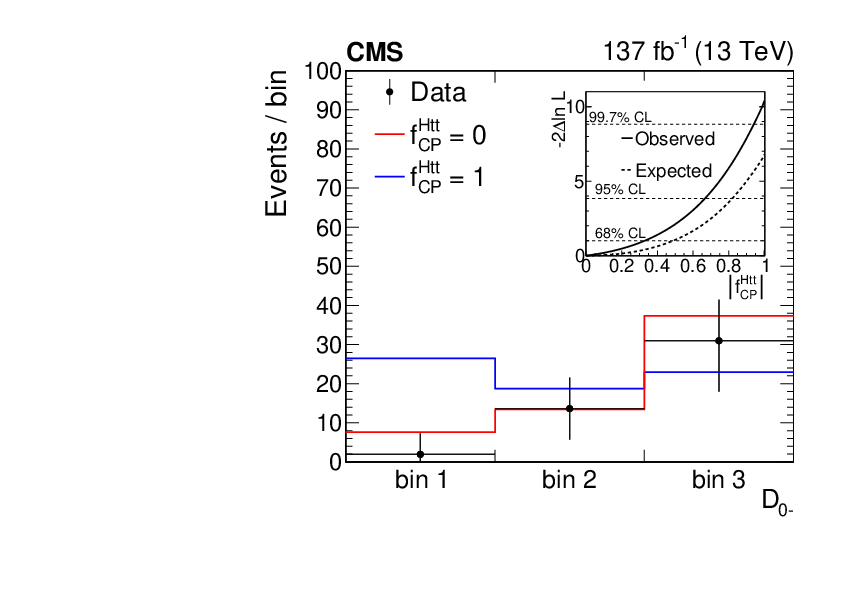
\includegraphics[width=\linewidth]{figures/tth/Figure_003.png}
    \caption{Distribution of events, weighted by S/(S+B), selected for the CP measurement of the Htt coupling. Events from both BDT-bkg categories in both the hadronic and leptonic channels are shown in each $\mathcal D_{0-}$ bin. The background contribution is subtracted from each bin. The likelihood scan for $f^{\text{Htt}}_{\text{CP}}$ is displayed in the inner panel. Taken from~\cite{tth_observation}.}
    \label{fig:tth_cp}
\end{figure}
The observed (expected) constraint on the CP structure of the Htt coupling is $f^{\text{Htt}}_{\text{CP}} = 0.00 \pm 0.33 (0.00 \pm 0.49)$ at 68\% CL.
The observed (expected) significance with which the pure CP-odd model is excluded is $3.2\sigma (2.6\sigma)$.
An additional systematic uncertainty is introduced for the CP measurement to account for potential differences in kinematic distributions obtained through the \textsc{JHUGen} generator and the \textsc{MadGraph} generator used to model the SM processes, though the uncertainty in the measurement is still dominated by the statistical uncertainty.

Thus, the measurement of the CP structure of the Htt coupling is found to be consistent with the SM value of $f^{\text{Htt}}_{\text{CP}} = 0$.

